%\documentclass[online, deutsch]{LEAthesis}
%\documentclass[deutsch]{LEAthesis}
%\documentclass[english]{LEAthesis}
%\documentclass[online,english]{LEAthesis}
\documentclass[english,diss]{LEAthesis}
%\documentclass[english,diss,final]{LEAthesis}

% %% Data for Bachelor/Master
% \title{Really a Very Very Extremely Long Title for Such a Thesis}
% \shorttitle{Title in Short}
% \author{Me Myself}
% \thesistype{Master Thesis}
% \thesisnr{MA0815}
% \matrnr{08193784}
% \supervisora{Prof. Dr.-Ing. Joachim Böcker}
% \supervisorb{Prof. Dr.-Ing. N.N.}
% \filingdate{\today}

%% Data for Dissertation
\title{Really a Very Very Extremely Long Title for Such a Thesis}
\shorttitle{Title in Short}
\author{Me Myself}
\supervisora{Prof. Dr.-Ing. Joachim Böcker}
\supervisorb{Prof. Dr.-Ing. N.N.}
\birthdate{30.02.1999}
\birthplace{Hintertupfingen}
\examdate{31.02.2025}
\thesisnr{333}
\publicationyear{2030}

\bibliography{references.bib}

%% additional definitions here


\newacronym{relu}{ReLU}{rectified linear unit}

\newacronym{lm}{LM}{Levenberg-Marquardt}
\newacronym{mse}{MSE}{mean squared error}
\newacronym{sgd}{SGD}{stochastic gradient descent}
\newacronym{nag}{NAG}{Nesterov accelerated gradient}
\newacronym{adam}{Adam}{adaptive moment estimation}


\newacronym{pca}{PCA}{principal component analysis}

\newacronym{psms}{PSMS}{particle swarm model selection}
\newacronym{pso}{PSO}{particle swarm optimization}

\newacronym{pc2}{PC\textsuperscript{2}}{Paderborn Center for Parallel Computing}
\newacronym{chp}{CHP}{combined heat and power}

 %Place acronyms here
\newacronym{pmsm}{PMSM}{permanent magnet synchronous motor}

\newacronym{fea}{FEA}{Finite-Element Analysis}
\newacronym{cfd}{CFD}{Computational Fluid Dynamics}
\newacronym{lptn}{LPTN}{lumped-parameter thermal network}

\newacronym{hmm}{HMM}{hidden Markov model}

\newacronym{mlp}{MLP}{Multi Layer Perceptron}
\newacronym{ann}{ANN}{artificial neural networks}
\newacronym{dnn}{DNN}{deep neural network}
\newacronym{fnn}{FNN}{feedforward neural network}
\newacronym{rnn}{RNN}{recurrent neural network}
\newacronym{brnn}{BRNN}{bidirectional recurrent neural network}
\newacronym{bptt}{BPTT}{backpropagation through time}
\newacronym[longplural={Long Short-Term Memories}]{lstm}{LSTM}{Long Short-Term Memory}
\newacronym[longplural={bidirectional Long Short-Term Memories}]{blstm}{BLSTM}{bidirectional Long Short-Term Memory}
\newacronym[longplural={general Long Short-Term Memories}]{lstmg}{LSTM-g}{General Long Short-Term Memory}
\newacronym{tdnn}{TDNN}{time-delay neural network}
\newacronym{narx}{NARX}{nonlinear autoregressive exogenous model}
\newacronym{cnn}{CNN}{convolutional neural network}
\newacronym{ntm}{NTM}{neural Turing machine}
\newacronym{gru}{GRU}{gated recurrent unit}

\newglossaryentry{CHPg}{name={Combined Heat and Power},description={Generator with heat recovery}}


 %Place glossary entries here

\begin{document}

\maketitle              

\frontmatter
    \makedeclaration
    \begin{abstract}

%This should include the tasks of your work, your achievements and a few words about the scientific domain where your work is positioned.
The safe operation of permanent magnet synchronous motors is heavily dependent on the heat development inside...


\end{abstract}
    \tableofcontents
    
\mainmatter

    \chapter{Introduction}
\label{cha:introduction}

%In der Einleitung sollte zunächst klar das Ziel der Arbeit genannt werden. (purpose)
The purpose of this thesis is primarily to investigate ...

%Anschließend sollte eine kurze Einordnung der Arbeit in den Kontext der aktuellen Forschung erfolgen. (motivation)

%Als letzter Absatz wird die Struktur der Arbeit erläutert (Sehr kurz und grob!) (scope)
This thesis is structured as follows...


\section{cite}

This is an example citation \cite{WaBo2016}. This is another example citation \cite{wallscheid2014real}.

You can also combine them as \cite{WaBo2016,wallscheid2014real}.


\section{wording}
Pay attention to the choice of words!
\begin{itemize}
	\item Switching work instead of switching energy!
\end{itemize}

\section{Upper and Lower Case}
\begin{itemize}
    \item Capitalize everything in headings except filler words like and, or, ....
    \item In captions, capitalize only the beginning of the sentence.
\end{itemize}



    \chapter{Software Overview} 

\section{Overview of Open Source Multi-platform Programs}
\begin{itemize}
	\item KiCAD (Linux, Mac, Windows)
	\item Inkscape (Linux, Mac, Windows) (Power electronics library provided by LEA can be found on \href{https://github.com/upb-lea/Inkscape_electric_Symbols}{https://github.com/upb-lea/Inkscape\_electric\_Symbols})
	\item Ganttproject (Linux, Mac, Windows) (Organizing software)
	\item GeckoCIRCUITS (Schematic simulator like LTSpice) (Java application for Linux, Mac, Windows) For controlling geckoCIRCUITS out of python, \href{https://github.com/tinix84/gecko/releases/tag/v1.1}{this} version is recommended.
	\item ONELAB (Linux, Mac, Windows) (FEM simulation tool. \href{https://onelab.info/}{Link})
	\item PyCharm (Linux, Mac, Windows) (Python programming editor)
	\item \href{https://github.com/upb-lea/transistordatabase}{Transistordatabase} (Transistor managing tool)
	\item \href{https://github.com/upb-lea/FEM_Magnetics_Toolbox}{FEM Magnetics Toolbox} (automated inductor / transformer design)
\end{itemize}

\section{Other programs, often used, propretary license}
\begin{itemize}
	\item Visio (Windows)
	\item Altium (Windows). \href{https://resources.altium.com/p/getting-started-pcb-design}{Altium tutorial}, \href{https://www.youtube.com/playlist?app=desktop&list=PLXvLToQzgzdfKKQn2wmpuSXz6sROQmO6R}{YT Playlist}. \href{https://altiumlibrary.com/}{Footprints}, \href{https://www.we-online.com/web/en/leiterplatten/produkte_/multilayer_leiterplatten/aufbauten_1/aufbauten_altium_1/aufbauten_4.php}{Layer-stackups}
	\item SolidWorks (Windows)
	\item ANSYS Student 20xxRx (Windows) \href{https://www.ansys.com/de-de/academic/free-student-products}{ANSYS Homepage} 
\end{itemize}
    \chapter{Example Chapter using Formulars, Tables and Figures} 
\label{cha:derivation}
%In diesem Kapitel kann das Modell vorgestellt werden, was erarbeitet oder bearbeitet wurde.
%%Purpose, Choice of NNs, Risk

\section{Programming Framework}
\label{sec:framework}
Deciding for a framework one can choose from several options, each having its own characteristics...

\section{Preprocessing and Feature Engineering}
\label{sec:features}
The data, which represents this work's investigative base, was gathered on a test bench having a three-phase \gls{pmsm} mounted with eight pole pairs.
The sample frequency was set to half a second consistently throughout the entire measurement. 
All parameters were received via first-order time-delay elements and a delay time $T_n$ of \SI{1.5}{\second}.
Moreover, ...

\tabref{tab:params} summarizes the parameters taken into account.
\begin{table}
	\caption{Considered input and target parameters.}
	\label{tab:params}
	\centering
	\begin{tabular}{l c c}
		\toprule
		parameter name & symbol & model position \\
		\midrule
		ambient temperature & $\vartheta_\mathrm{a}$ & input \\
		liquid coolant temperature & $\vartheta_\mathrm{c}$ & input \\
		actual voltage $d$-axis component & $u_\mathrm{d}$ & input \\
		actual voltage $q$-axis component & $u_\mathrm{q}$ & input \\
		actual current $d$-axis component & $i_\mathrm{d}$ & input \\
		actual current $q$-axis component & $i_\mathrm{q}$ & input \\
		\hline
		permanent magnet temperature & $\vartheta_{\mathrm{PM}}$ & output \\
		stator teeth temperature & $\vartheta_{\mathrm{ST}}$ & output \\
		stator winding temperature & $\vartheta_{\mathrm{SW}}$ & output \\
		stator yoke temperature & $\vartheta_{\mathrm{SY}}$ & output\\
		\bottomrule
	 \end{tabular}
\end{table}


\subsection{Normalization}
\label{subsec:normalization}
In this work, a simple normalization scheme is conducted.
If $x^{(t)}$ denotes the true value of a parameter $X$ to the time $t$ and $\bar{x} = \mu(X) = \frac{1}{N}\sum\nolimits_{t, i} x^{(t)}_i$ represents the sample mean of this parameter over each considered profile $i\in I$ while the parameters' unbiased sample standard deviation is computed by $\sigma(X)=\sqrt{(N-1)^{-1}\sum\nolimits_{t, i} (x^{(t)}_i - \bar{x})^2}$, then the normalized value $x_\text{norm}$ is calculated by  
\begin{equation}
	x_\text{norm}^{(t)} = \frac{x^{(t)}-\bar{x}}{\sigma(X)}.
\end{equation}
\nomenclature[xnormt]{$x_\text{norm}^{(t)}$}{normalized value}	

Equations can also be aligned:
\begin{align}
    a&=b+c\\
    \begin{split}
        \dot{x}_2(t)&= \frac{1}{C_2} \left( i_1(t)-i_2(t)\right)= \frac{1}{C_2} \left[ \frac{1}{R_1} \left(u(t)-x_2(t)-x_1(t) \right)-\frac{1}{R_2} x_2(t)\right]\\
        &= \frac{1}{C_2 R_1} u(t)-\frac{1}{C_2 R_1} x_1(t) - \frac{1}{C_2} \left( \frac{1}{R_1}+\frac{1}{R_2}\right) x_2(t). 
        \label{eq:splitline}
    \end{split}
\end{align}

In \eqref{eq:splitline} the equation was split into two lines. Use this for long equations.

\section{Architecture}
\label{sec:architecture}
According to \figref{fig:cnn}, the model topology comprises...

\begin{figure}[htb]
	\centering
    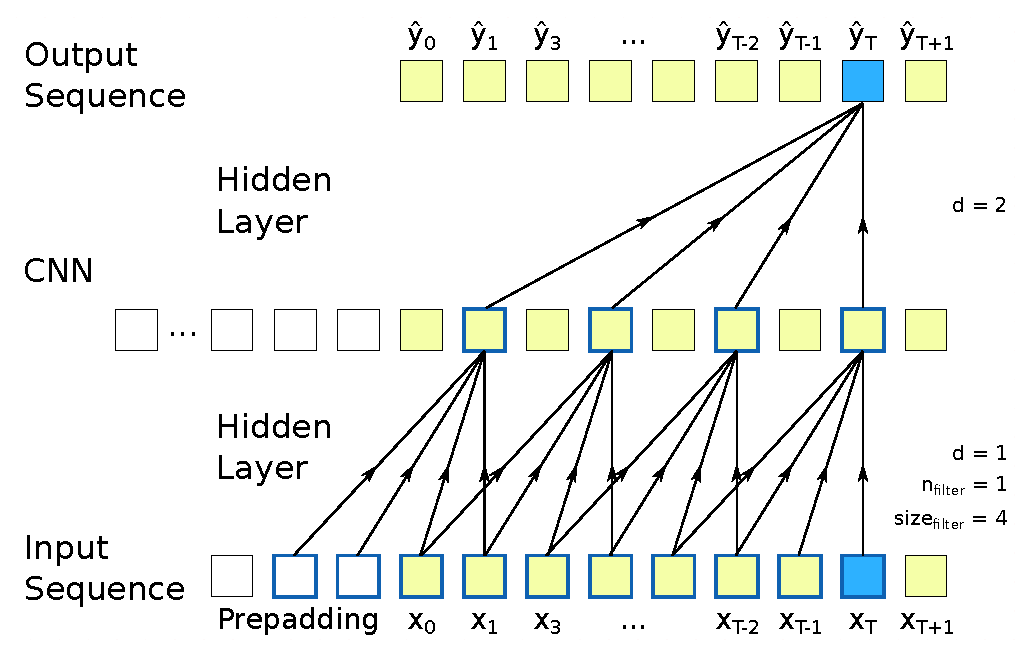
\includegraphics[width=0.75\textwidth]{modeling/CNN_over_sequence.eps}
    \caption{Convolutional Neural Network.}
	\label{fig:cnn}
\end{figure}



    \chapter{Plotting Examples Using Different Programs} 
\label{cha:evaluation}

\section{Plotting with tikz}

See the example \figref{fig:tikz_example_01}
\begin{figure}[ht]
    \centering
    \begin{center}

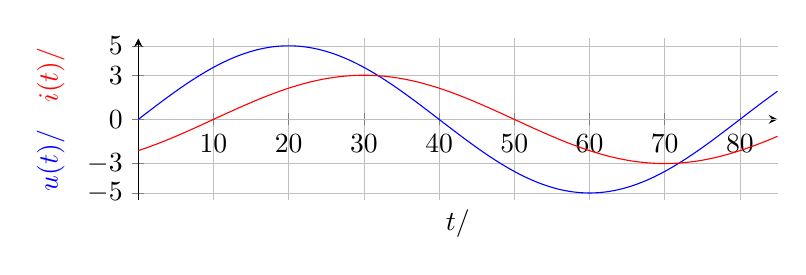
\begin{tikzpicture}
    \begin{axis}[
        domain=0:85,
        xmin=0, xmax=85,
        ymin=-5.5, ymax=5.5,
        samples=500,
        axis y line=center,
        axis x line=middle,
        xtick distance=10,
        ytick distance=1,
        extra y ticks=0,
        width=.8\textwidth,
        height=.3\textwidth,
        x label style={at={(axis description cs:0.5,0)},anchor=north},
        y label style={at={(axis description cs:-.1,.5)},rotate=90,anchor=south},
        ytick={-5,-3,0,3,5},
%         yticklabels={$-2 u_0$, $2 u_0$},
        xlabel={$t/\ms$},
         ylabel={{\color{blue}$u(t)/\volt$}\quad{\color{red}$i(t)/\ampere$}},
        grid=both,
        grid style={line width=.1pt, draw=gray!10},
        major grid style={line width=.2pt,draw=gray!50}    ]
        \addplot+[color=blue,mark=none] {5*sin(deg(x/80*6.283))};
        \addplot+[color=red,mark=none] {3*sin(deg((x-10)/80*6.283))};
    \end{axis}
\end{tikzpicture}
\end{center}
    \caption{Example of a tikz figure}
    \label{fig:tikz_example_01}
\end{figure}
\begin{figure}[ht]
    \centering
    \begin{center}
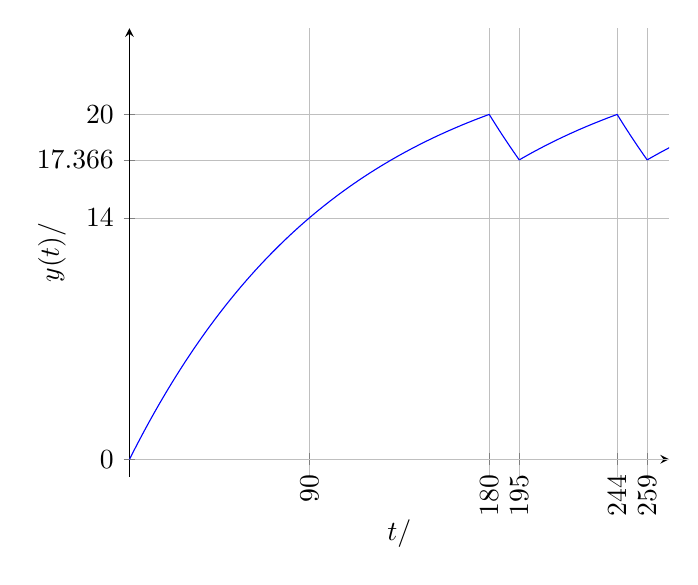
\begin{tikzpicture}
    \begin{axis}[
        domain=0:270,
        xmin=0, xmax=270,
        ymin=-1, ymax=25,
        samples=500,
        axis y line=center,
        axis x line=middle,
        %xtick distance=1,
        %ytick distance=1,
        extra y ticks=0,
        x label style={at={(axis description cs:0.5,-.075)},anchor=north},
        y label style={at={(axis description cs:-.1,.5)},rotate=90,anchor=south},
        xlabel={$t/\minute$},
        ylabel={$y(t)/\celsius$},
        ytick={0,14,17.366,20},
        xtick={0, 90, 180, 195,  244,  259},
        xticklabels={0, 90, 180, 195,  244,  259},
        xticklabel style={rotate=90},
        yticklabels={0,14,17.366,20},
        grid=both,
        grid style={line width=.1pt, draw=gray!10},
        major grid style={line width=.2pt,draw=gray!50},    ]
        \addplot+[color=blue,mark=none,domain=0:180] {2000*0.01225*(1-exp(-x/106.22))};
        \addplot+[color=blue,mark=none,domain=180:195] {20*(exp(-(x-180)/106.22))};
        \addplot+[color=blue,mark=none,domain=195:244] {2000*0.01225*(1-exp(-(x-64)/106.22))};
        \addplot+[color=blue,mark=none,domain=244:259] {20*(exp(-(x-244)/106.22))};
        \addplot+[color=blue,mark=none,domain=259:300] {2000*0.01225*(1-exp(-(x-128)/106.22))};
    \end{axis}
\end{tikzpicture}
\end{center}
    \caption{Example of another tikz figure}
    \label{fig:tikz_example_02}
\end{figure}
\begin{figure}[ht]
    \centering
    \begin{center}
\begin{tikzpicture}
    \begin{axis}[
        domain=0:300,
        xmin=0, xmax=300,
        ymin=-1, ymax=2200,
        samples=500,
        axis y line=center,
        axis x line=middle,
        %xtick distance=1,
        %ytick distance=1,
        extra y ticks=0,
        x label style={at={(axis description cs:0.5,-.075)},anchor=north},
        y label style={at={(axis description cs:-.1,.5)},rotate=90,anchor=south},
        xlabel={$t/\minute$},
        ylabel={$u(t)/\watt$},
        xtick={0, 90, 180, 195,  244,  259},
        xticklabels={0, 90, 180, 195,  244,  259},
        xticklabel style={rotate=90},
        ytick={0,2000},
        yticklabels={0,2000},
        %yticklabels={$-2 u_0$,$-u_0$, $0$,$\frac{u_0}{2}$, $u_0$},
        grid=both,
        grid style={line width=.1pt, draw=gray!10},
        major grid style={line width=.2pt,draw=gray!50},    ]
        \addplot[color=blue,mark=none] coordinates{
            ( 0,  2000)
            (180,  2000)
            (180,  0)
            (195,  0)
            (195,  2000)
            (244,  2000)
            (244,  0)
            (259,  0)
            (259,  2000)
            (300,  2000)
    };
    \end{axis}
\end{tikzpicture}
\end{center}
    \caption{Example of even another tikz figure}
    \label{fig:tikz_example_03}
\end{figure}



\section{Circuits with circuitikz}
See the following example \figref{fig:circuitikz_example}.
\begin{figure}[ht]
    \centering
    \begin{center}
\begin{circuitikz}
	\draw
	(0,0)
	to [short,o-*] ++(0,-.5) coordinate(up1) 
	(up1) to [short,-] ++(-1,0)  coordinate(up1l) 
	(up1) to [short,-] ++(1,0)  coordinate(up1r)
	(up1) ++(0,-2) coordinate(mid1o)
	(mid1o) to [short,-] ++(-1,0)  coordinate(mid1ol) 
	(mid1o) to [short,-] ++(1,0)  coordinate(mid1or)
	(mid1o) to [short,*-*] ++(0,-.5) coordinate(mid1u) 
	(mid1u) ++(0,-2) coordinate(down1)
	(mid1u) to [short,-] ++(-1,0)  coordinate(mid1ul) 
	(mid1u) to [short,-] ++(1,0)  coordinate(mid1ur)
	(down1) to [short,-] ++(-1,0)  coordinate(down1l) 
	(down1) to [short,-]  ++(1,0)  coordinate(down1r)
	(down1) to [short,*-o] ++(0,-.5) 
	(up1l) to [L,l^=$L$,v=$U_\text{L}$,mirror] (mid1ol)
	(up1r) to [R=$R$] (mid1or)
	(mid1ul) to [C,l_=$C$] (down1l)
	(mid1ur) to [R=$R$] (down1r)

        (5,0)
	to [short,o-*] ++(0,-.5) coordinate(up2) 
	(up2) to [short,-] ++(-1,0)  coordinate(up2l) 
	(up2) to [short,-] ++(1,0)  coordinate(up2r)
	(up2) ++(0,-4) coordinate(down2)
	(down2) to [short,-] ++(-1,0)  coordinate(down2l) 
	(down2) to [short,-]  ++(1,0)  coordinate(down2r)
	(down2) to [short,*-o] ++(0,-.5) 
	(up2l) to [R,l^=$R$,i=$i_\text{R}$] ++(0,-2) to  [C,l_=$C$] (down2l)
	(up2r) to [R=$R$] ++(0,-2) to [L,l^=$L$] (down2r)
	;
\end{circuitikz}

\end{center}

    \caption{Example of a circuitikz figure}
    \label{fig:circuitikz_example}
\end{figure}


And this is not about \acrshort{CHP} or \gls{CHPg}

\section{Circuits with Inkscape Library}
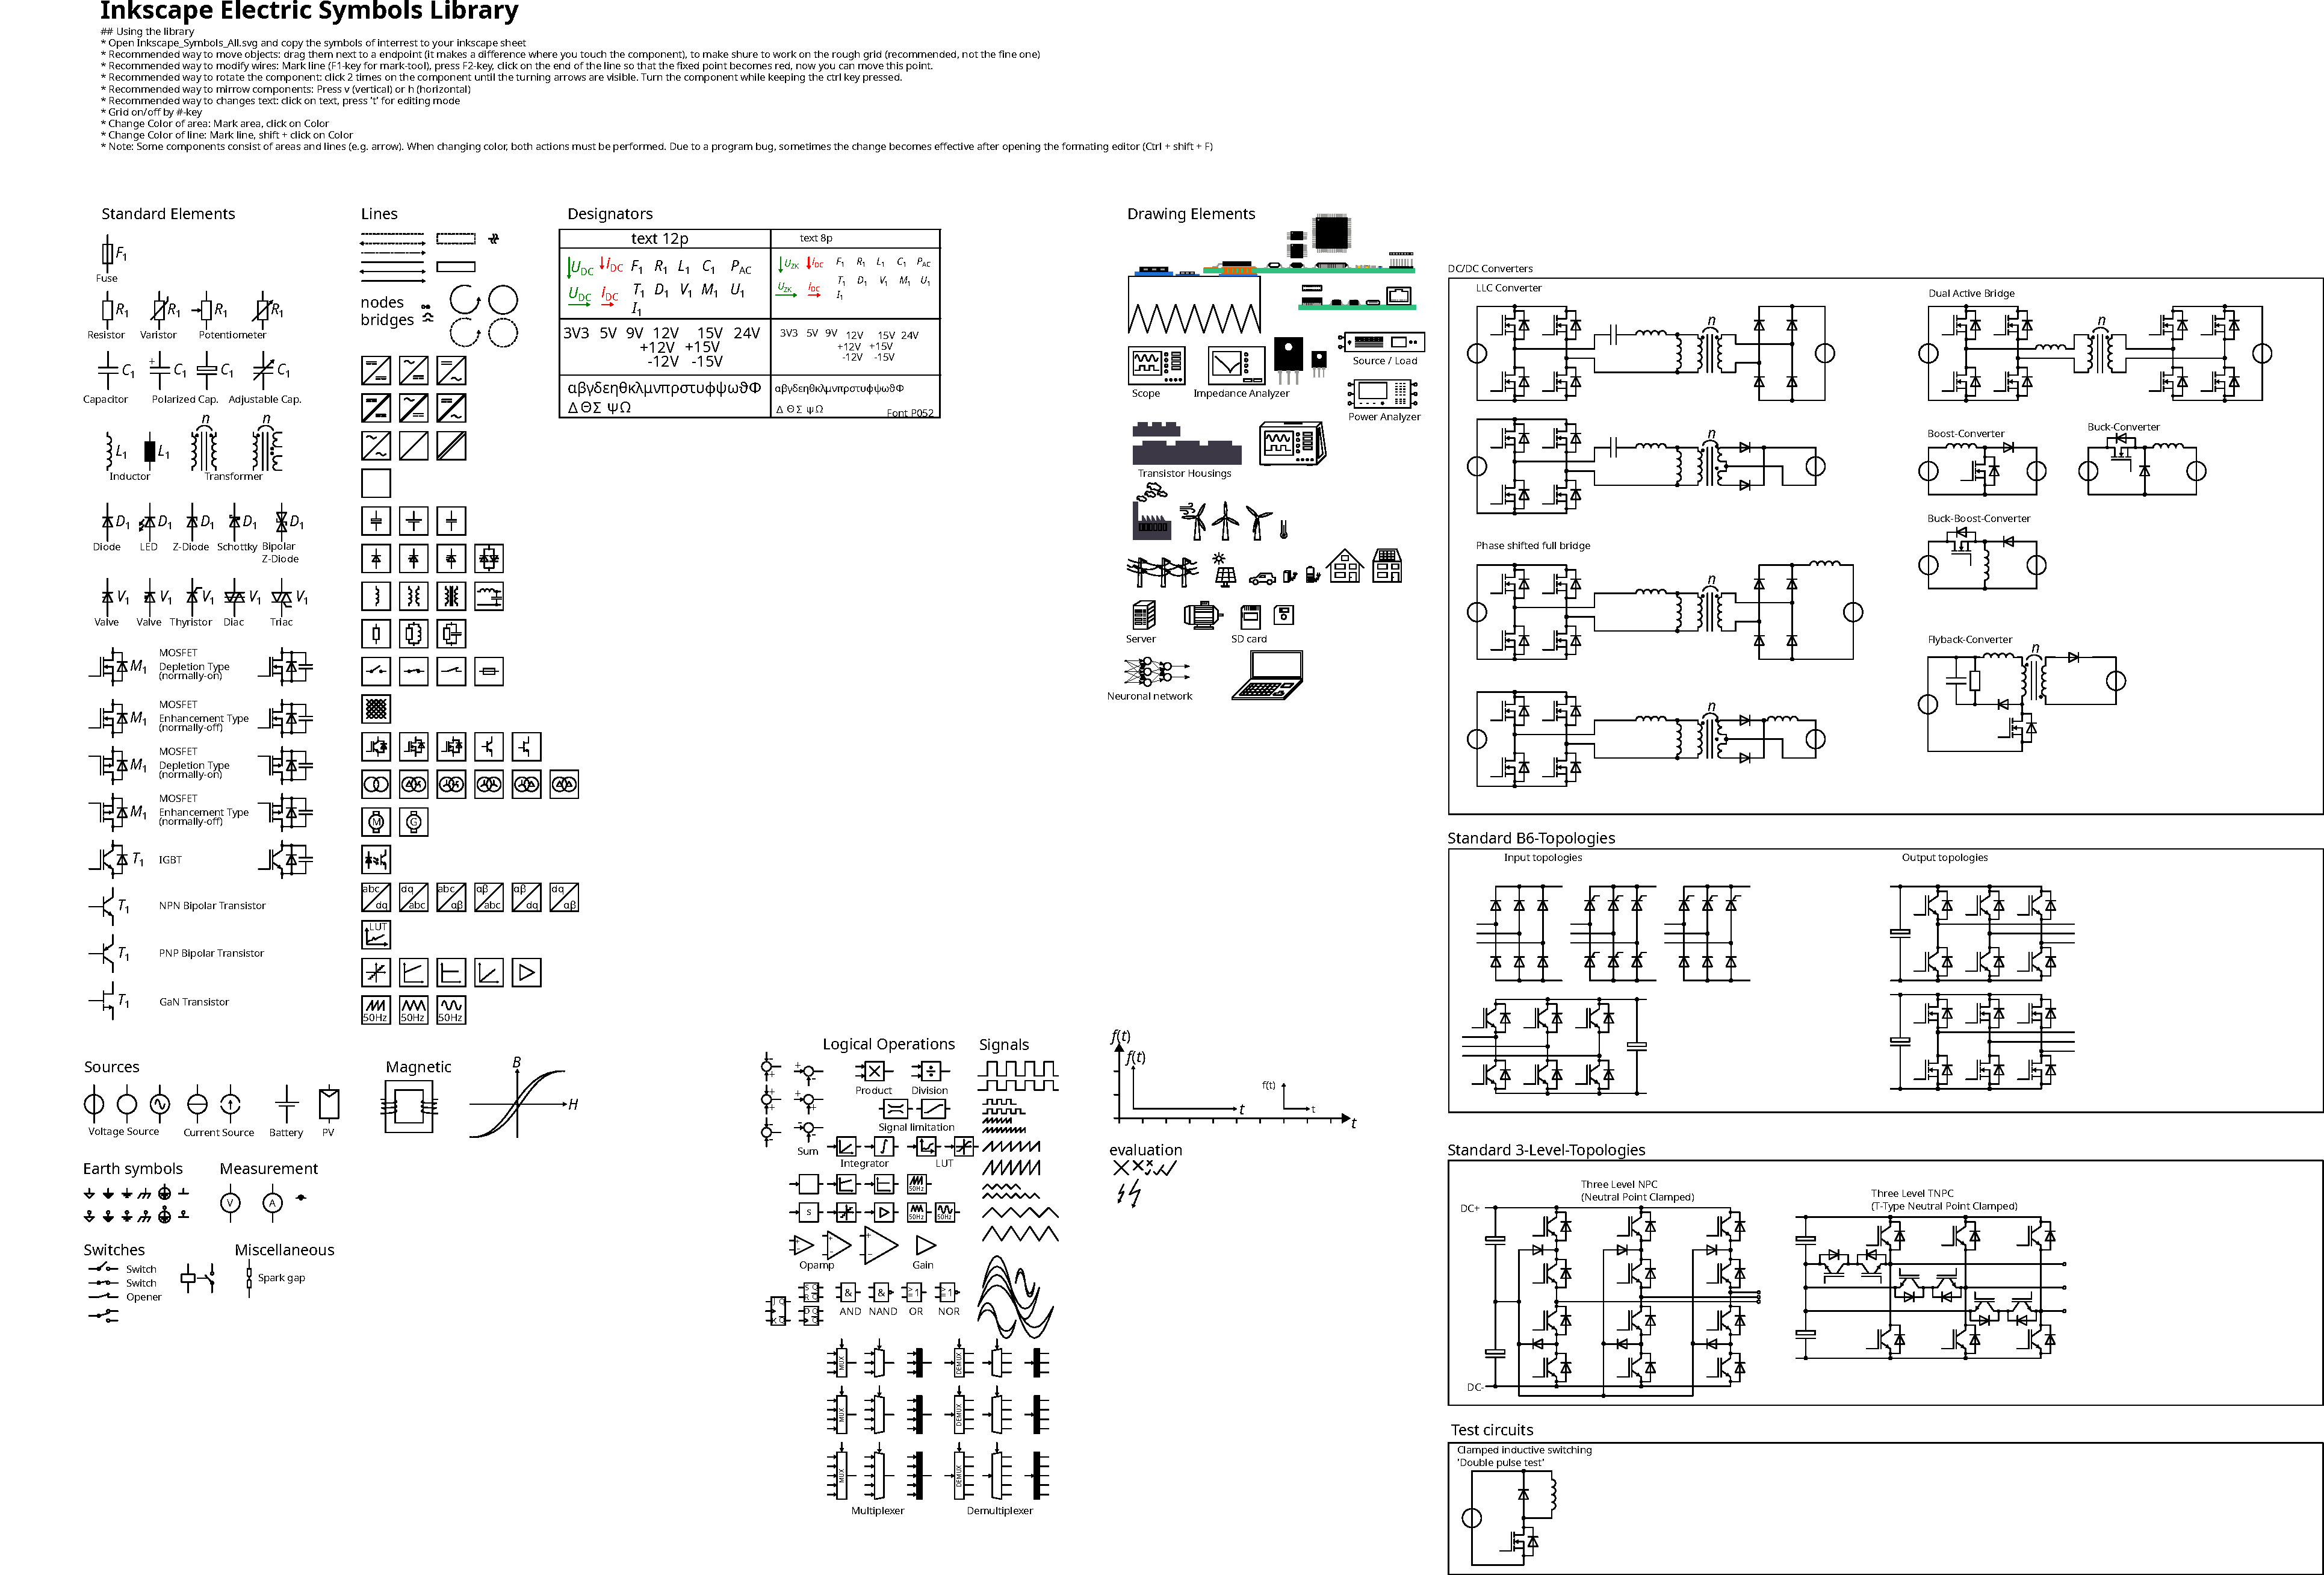
\includegraphics[]{fig/inkscape/Inkscape_Symbols_All.pdf}
There is an Inkscape template for power electronics symbols provided by LEA, hosted on Github. \href{https://github.com/upb-lea/Inkscape_electric_Symbols}{https://github.com/upb-lea/Inkscape\_electric\_Symbols}.


    \chapter{Conclusion} 
\label{cha:conclusion}

This work's intention was the investigation of...

\section{Future Work}

During the course of this thesis, some perspectives loomed for future investigations...


\section{Publish your work}
You can optionally publish your work through the university library. Visit the following link: \href{https://digital.ub.uni-paderborn.de/ubpb}{https://digital.ub.uni-paderborn.de/ubpb}.

\backmatter
    
    \appendix
\label{cha:appendix}

In this chapter all remaining plots regarding the hyper-parameter optimizations are depicted for the sake of completeness...


\section{First Appendix Section}

hello

\section{Second Appendix Section}

hello
    \lists

    \ifdiss\iffinal\else\pagestyle{empty}
\chapter{Lebenslauf}
\label{sec:Lebenslauf}
%\vskip-22ex
\begin{tabular}{ll}
  Name 				& Mustermann \\
  Vorname 		& Max \\
  Wohnort			& Paderborn \\
  Geburtsdatum/-ort	& 30.02.1988 in Paderborn \\
  Nationalität & deutsch  \\
  Familienstand & ledig \\[2ex]
  \textbf{Schulbildung} 	&  \\
  09/1988 - 07/1992	& Grundschule \\
  08/1992 - 01/1999 & Gymnasium \\[2ex]
  \textbf{Wehrdienst} 		&  \\
  02/2000 - 09/2001 & wenn es den noch gab \\[2ex]
  \textbf{Studium} 	&  \\
  10/2001 - 04/2009 & Universität Paderborn\\[2ex]
  \multicolumn{2}{l}{\textbf{Wissenschaftliche Tätigkeit} }	 \\
  seit 09/2010			& Universität Paderborn, Fachgebiet LEA \\[2ex]
  \textbf{Beruf} 		&  \\
  12/2009 - 04/2010 & Firma Mustermann, Paderborn \\[2ex]
  \textbf{Sprachkenntnisse} 		&  Deutsch \\
 					&  Englisch \\[2ex]

 Paderborn, \today &\\[10ex]
\end{tabular}

\textbf{Drei Stichworte für den Deutschen Fakultätentag zur Dissertation}
  \begin{itemize}
   \item Eins
   \item Zwei
   \item Drei
  \end{itemize}
\fi\fi
\end{document}
